\documentclass[11pt,a4paper]{article}

\usepackage[margin=2.4cm]{geometry}
\usepackage{fontspec}
\usepackage{xeCJK}
\usepackage{booktabs}
\usepackage{amsmath}
\usepackage{tabularx}
\usepackage{array}
\usepackage{float}
\usepackage{graphicx}
\usepackage{enumitem}
\usepackage{xcolor}
\usepackage{microtype}
\usepackage{fancyhdr}
\usepackage[hidelinks]{hyperref}

\IfFontExistsTF{PingFang TC}{
  \setCJKmainfont{PingFang TC}
  \setCJKsansfont{PingFang TC}
}{
  \setCJKmainfont{Songti TC}
  \setCJKsansfont{Heiti TC}
}
\IfFontExistsTF{TeX Gyre Pagella}{\setmainfont{TeX Gyre Pagella}}{}

\definecolor{ink}{HTML}{17213A}
\definecolor{accent}{HTML}{9B772C}
\definecolor{soft}{HTML}{F4F1E8}
\definecolor{rulegray}{HTML}{C8C2B5}

\color{ink}
\pagecolor{white}
\setlength{\parindent}{0pt}
\setlength{\parskip}{0.65em}
\setlist[itemize]{leftmargin=1.5em,itemsep=0.25em,topsep=0.25em}
\renewcommand{\arraystretch}{1.22}
\newcolumntype{Y}{>{\raggedright\arraybackslash}X}
\newcolumntype{L}[1]{>{\raggedright\arraybackslash}p{#1}}

\pagestyle{fancy}
\fancyhf{}
\fancyfoot[C]{\small\thepage}
\renewcommand{\headrulewidth}{0pt}
\fancypagestyle{plain}{%
  \fancyhf{}%
  \fancyfoot[C]{\small\thepage}%
  \renewcommand{\headrulewidth}{0pt}%
}

\newcommand{\sectionrule}{\par\vspace{-0.45em}{\color{accent}\rule{\linewidth}{0.8pt}}\vspace{0.4em}}
\newcommand{\dataterm}[1]{\texttt{#1}}
\graphicspath{{../figures/}}

\begin{document}
\hypersetup{pdftitle={Answers - Parts 1 to 5}}
\pagestyle{fancy}

\begin{center}
  {\color{accent}\large PART 1}\par
  \vspace{0.25em}
  {\Large\bfseries Prepare the Data for Classification}\par
\end{center}

\vspace{0.8em}

\section*{1. Classification Task}
\sectionrule

我使用 \dataterm{penguins\_raw.csv} 中的資料進行多類別分類。資料裡的每一列都可以看成一個 data object，代表一隻接受觀測的成年企鵝，記錄了採樣地點、時間、身體測量值與實驗資訊。原始資料共有 344 筆觀測與 17 個欄位。

要預測的 class label 是 \dataterm{Species}，共有 Adelie、Chinstrap 與 Gentoo 三個類別。模型會根據企鵝的身體測量值，判斷它屬於哪一個物種。後面的 KNN 與 Decision Tree 都會沿用這裡選出的 features，也會共用同一組 train/test split，讓兩個模型可以在相同基準下比較。

\section*{2. Feature Selection}
\sectionrule

\subsection*{納入的 features}

我最後選了四個 numerical attributes。這些欄位都直接描述企鵝的外部形態，單位清楚，在進行分類時也合理可取得。另一方面，四個欄位的數值尺度並不相同，剛好可以在 Part 2 觀察 proximity 與 scaling 會如何影響 KNN。

\begin{table}[H]
\centering
\small
\begin{tabularx}{\linewidth}{L{4.0cm}L{2.2cm}Y}
\toprule
\textbf{原始欄位} & \textbf{型態／單位} & \textbf{納入理由} \\
\midrule
Culmen Length (mm) & numerical / mm & 喙長是物種形態差異的重要描述。 \\
Culmen Depth (mm) & numerical / mm & 喙深與喙長互補，可協助區分相近物種。 \\
Flipper Length (mm) & numerical / mm & 鰭肢長反映體型與物種形態。 \\
Body Mass (g) & numerical / g & 體重提供整體體型資訊，但尺度明顯大於毫米欄位。 \\
\bottomrule
\end{tabularx}
\end{table}

\clearpage
\pagestyle{fancy}
\subsection*{未納入的 attributes}

\begin{table}[H]
\centering
\small
\begin{tabularx}{\linewidth}{L{4.2cm}Y}
\toprule
\textbf{欄位} & \textbf{排除理由} \\
\midrule
Species & 要預測的 label，不可同時作為 feature。 \\
studyName、Sample Number、Individual ID & 採樣與識別資訊；代碼本身沒有可泛化的生物意義，也可能使模型記住研究批次。 \\
Region、Stage & 兩欄在資料中各只有一個值，沒有分類資訊。 \\
Island & 地點與物種分布高度相關，容易形成 location shortcut；這裡希望模型根據企鵝本身的形態分類，因此排除。 \\
Clutch Completion、Date Egg & 繁殖與採樣時間資訊，和個體形態分類的目的較遠。 \\
Sex & 有 11 筆缺失，且為 categorical attribute。Part 2 將專注比較 numerical proximity 與 scaling，所以不納入。 \\
Delta 15 N、Delta 13 C & 分別缺失 14 與 13 筆，且依賴實驗室分析；不一定是實際分類時可立即取得的資訊。 \\
Comments & 自由文字採樣備註，290 筆缺失，內容也不是穩定的個體特徵。 \\
\bottomrule
\end{tabularx}
\end{table}

\section*{3. Data Quality}
\sectionrule

\subsection*{Missing values}

原始 CSV 使用字串 \dataterm{NA} 表示缺失。我檢查後發現 label 沒有缺失；四個入選 features 則各缺 2 筆，而且都集中在相同的兩筆觀測：一筆 Adelie 與一筆 Gentoo 都缺少全部四個形態測量值。這 2 筆只占原始資料的 $2/344=0.58\%$，也沒有任何可用的形態資訊，因此我直接刪除這兩筆資料，不用四個平均數拼出一組虛構的個體形態。

\begin{table}[H]
\centering
\small
\begin{tabular}{lrr}
\toprule
\textbf{欄位群組} & \textbf{缺失筆數} & \textbf{處理} \\
\midrule
四個入選形態欄位 & 各 2 & 刪除共同缺失的 2 筆觀測 \\
Sex & 11 & 欄位未納入 \\
Delta 15 N / Delta 13 C & 14 / 13 & 欄位未納入 \\
Comments & 290 & 欄位未納入 \\
其餘欄位 & 0 & 無須處理 \\
\bottomrule
\end{tabular}
\end{table}

\subsection*{Outliers}

我用 Tukey rule 檢查四個入選 features：低於 $Q_1-1.5\,IQR$ 或高於 $Q_3+1.5\,IQR$ 的數值會先列為待檢查離群值。檢查結果顯示，四個欄位的觀測範圍都落在界線內，沒有發現離群值。因此這部分不刪除資料，也不需要 clipping 或 winsorization。

\begin{table}[H]
\centering
\small
\begin{tabular}{lrrr}
\toprule
\textbf{Feature} & \textbf{觀測範圍} & \textbf{IQR 合理範圍} & \textbf{離群筆數} \\
\midrule
Culmen Length (mm) & 32.1--59.6 & 25.31--62.41 & 0 \\
Culmen Depth (mm) & 13.1--21.5 & 10.95--23.35 & 0 \\
Flipper Length (mm) & 172--231 & 155.5--247.5 & 0 \\
Body Mass (g) & 2700--6300 & 1750--6550 & 0 \\
\bottomrule
\end{tabular}
\end{table}

\subsection*{Duplicate and inconsistent values}

我也針對重複值做了兩層檢查。先比較完整 17 欄，沒有發現完全重複的紀錄；刪除缺失列後，四個形態 features 也沒有相同的 feature vector。\dataterm{Individual ID} 單獨看會在不同研究批次中重複，所以不能把它當成整份資料的唯一鍵；改用 \dataterm{studyName + Species + Individual ID} 檢查後則沒有重複。這也進一步支持把識別欄位排除在模型之外。

類別值沒有前後空白或同義拼寫混用，但原始 \dataterm{Species} 的英文大小寫格式不一致，例如 ``Adelie Penguin'' 與 ``Gentoo penguin''。為了讓 label 簡潔一致，我將它們整理成 \dataterm{Adelie}、\dataterm{Chinstrap} 與 \dataterm{Gentoo}。這一步只統一顯示名稱，沒有合併或改變任何類別。

\section*{4. Final Data Preparation}
\sectionrule

整理資料時，我依序進行了以下步驟：

\begin{enumerate}[leftmargin=1.7em,itemsep=0.35em]
  \item 將原始字串 \dataterm{NA} 解析為 missing value。
  \item 明確選取四個形態 features 與 \dataterm{Species} label。
  \item 刪除四個入選 features 任一缺失的觀測，共 2 筆。
  \item 將三個物種 label 標準化為簡短且一致的名稱。
  \item 保留數值的原始單位，輸出 342 筆可供分類使用的資料。
\end{enumerate}

\begin{table}[H]
\centering
\small
\begin{tabular}{lr}
\toprule
\textbf{最終資料摘要} & \textbf{結果} \\
\midrule
可用觀測數 & 342 \\
Adelie & 151 \\
Chinstrap & 68 \\
Gentoo & 123 \\
Features & 4 個 numerical attributes \\
Label & species（3 classes） \\
\bottomrule
\end{tabular}
\end{table}

整理後的 feature matrix $X$ 包含 \dataterm{culmen\_length\_mm}、\dataterm{culmen\_depth\_mm}、\dataterm{flipper\_length\_mm} 與 \dataterm{body\_mass\_g}；target vector $y$ 為 \dataterm{species}。輸出檔另外保留 \dataterm{source\_row}，方便日後回頭查找原始 CSV 的資料列，但這個欄位不會輸入模型。

這個階段我先保留所有 feature 的原始單位，不做 scaling。Body Mass 的數值尺度遠大於其餘三欄，正好可以留到 Part 2 比較 preprocessing 前後的差異。進行 scaling 時，scaler 只會用 training set 擬合，再套用到 test set，避免 data leakage；train/test split、標準化與模型訓練也都留到 Part 2 一起處理。

\clearpage

\begin{center}
  {\color{accent}\large PART 2}\par
  \vspace{0.25em}
  {\Large\bfseries Chapter 2 應用：KNN Classification}\par
\end{center}

\vspace{1.0em}

\section*{1. Train/Test Split}
\sectionrule

這裡沿用 Part 1 整理出的 342 筆完整觀測，以及相同的四個 numerical features：culmen length、culmen depth、flipper length 與 body mass。要預測的 label 仍然是 species。

我使用 stratified train/test split，將 test size 設為 20\%，並固定 \dataterm{random\_state=42}。最後 training set 有 273 筆，test set 有 69 筆。採用分層抽樣，是希望三個物種在兩組資料中的比例都能接近原始分布。切分結果也已經依 \dataterm{source\_row} 保存，Part 4 的 Decision Tree 會直接沿用同一組 split。

\begin{table}[H]
\centering
\small
\begin{tabular}{lrrr}
\toprule
\textbf{Split} & \textbf{Adelie} & \textbf{Chinstrap} & \textbf{Gentoo} \\
\midrule
Training set & 121 & 54 & 98 \\
Test set & 30 & 14 & 25 \\
\bottomrule
\end{tabular}
\end{table}

\section*{2. KNN and Proximity Design}
\sectionrule

我用 Part 1 選出的四個 features 建立 KNN。三個設定都固定 $k=5$，並採用 majority vote（uniform weights），這樣就能把比較重點放在 proximity 與 preprocessing，而不會同時受到其他參數干擾。

對兩筆企鵝資料 $x$ 與 $z$，Euclidean distance 與 Manhattan distance 分別為
\[
d_2(x,z)=\sqrt{\sum_j(x_j-z_j)^2},
\qquad
d_1(x,z)=\sum_j\lvert x_j-z_j\rvert.
\]
Euclidean distance 可以理解成多維空間中的直線距離，對較大的座標差異也會比較敏感；Manhattan distance 則是把各 feature 的絕對差異加總起來。由於四個 features 都是 numerical attributes，兩種距離都能直接使用，也很適合拿來比較 proximity 設計的影響。

\section*{3. Preprocessing and Scaling Comparison}
\sectionrule

兩種 distance 都會受到 feature 尺度影響。資料中的 body mass 約為 2700--6300 g，數值範圍遠大於其他毫米欄位；如果直接計算 raw distance，體重很容易主導哪些企鵝會被視為鄰居。因此我把 scaling 前後的 KNN 放在一起比較。

Z-score standardization 使用
\[
z_j=\frac{x_j-\mu_j^{(train)}}{\sigma_j^{(train)}}.
\]
其中的平均數與標準差只用 training set 估計，再套用到 test set。程式以 \dataterm{Pipeline} 封裝 scaler 與 KNN，確保 preprocessing 的擬合過程不會先看到 test data。

我安排了以下三個設定：

\begin{enumerate}[leftmargin=1.7em,itemsep=0.35em]
  \item Raw Euclidean：保留原始單位，使用 Euclidean distance。
  \item Z-score Euclidean：先做 Z-score，再使用 Euclidean distance；與設定 1 隔離 scaling 的影響。
  \item Z-score Manhattan：維持相同 scaling，改用 Manhattan distance；與設定 2 隔離 proximity metric 的影響。
\end{enumerate}

\section*{4. Accuracy and Confusion Matrix}
\sectionrule

\begin{table}[H]
\centering
\small
\begin{tabularx}{\linewidth}{L{3.7cm}L{2.4cm}Yrr}
\toprule
\textbf{設定} & \textbf{Scaling} & \textbf{Proximity} & \textbf{正確筆數} & \textbf{Accuracy} \\
\midrule
Raw Euclidean & 無 & Euclidean ($p=2$) & 51 / 69 & 73.91\% \\
Z-score Euclidean & StandardScaler & Euclidean ($p=2$) & 69 / 69 & 100.00\% \\
Z-score Manhattan & StandardScaler & Manhattan ($p=1$) & 69 / 69 & 100.00\% \\
\bottomrule
\end{tabularx}
\end{table}

我選擇 Raw Euclidean 作為代表性設定。雖然它的 accuracy 最低，錯誤分布卻最能看出未處理尺度時，KNN 的 proximity 會受到什麼影響。其 error rate 為
\[
1-\text{accuracy}=1-\frac{51}{69}=\frac{18}{69}=26.09\%.
\]

\begin{figure}[H]
\centering
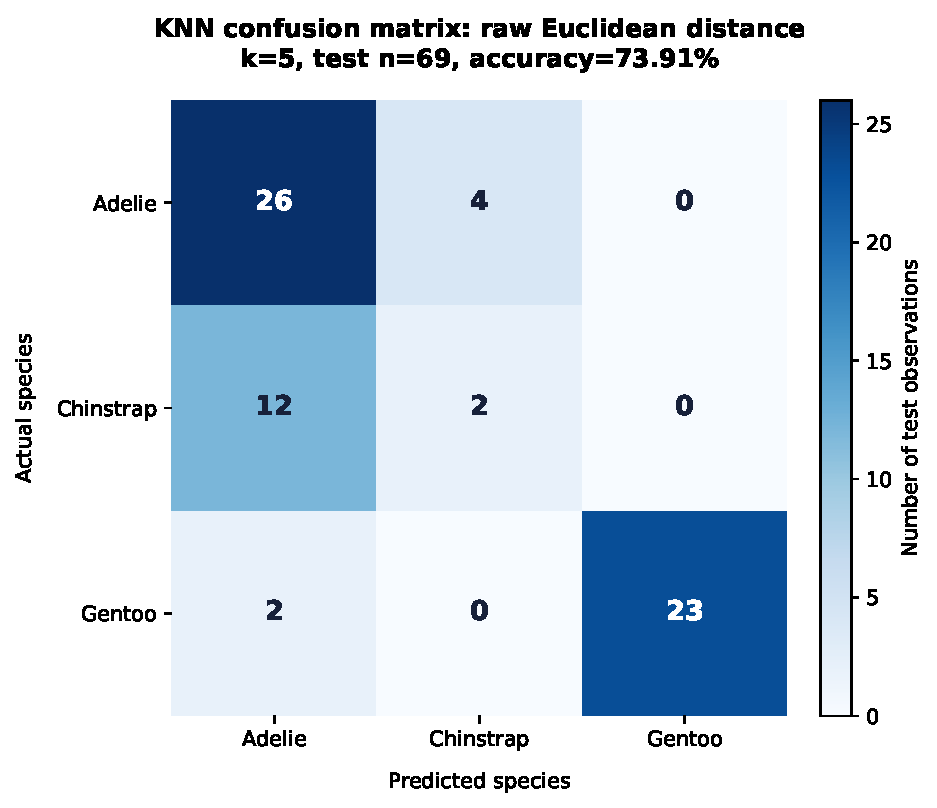
\includegraphics[width=0.62\linewidth]{part2_knn_confusion_matrix.pdf}
\caption{Raw Euclidean KNN 在 test set 的 confusion matrix。列為 actual class，欄為 predicted class。}
\end{figure}

\clearpage
\section*{5. Comparison and Discussion}
\sectionrule

從 confusion matrix 可以先看到，Raw Euclidean 對 14 筆 Chinstrap 只判對 2 筆，其中 12 筆被判成 Adelie；另外還有 4 筆 Adelie 被判成 Chinstrap。Gentoo 的辨識相對穩定，25 筆中判對 23 筆。這和尺度主導的預期一致：raw distance 大量受到 body mass 影響，喙部形態帶來的物種差異相對被壓低，所以 Adelie 與 Chinstrap 特別容易混淆。

做完 Z-score 後，四個 features 都改以各自的標準差為單位，Euclidean 設定在這組 test set 上將 69 筆全部判對。換句話說，scaling 確實改變了鄰居的組成，而且這個差異剛好修正了 raw distance 的 18 筆錯誤。StandardScaler 只用 training set 擬合，所以這項改善沒有使用 test label 或 test distribution 的資訊。

在相同的 Z-score preprocessing 下，Euclidean 與 Manhattan 得到完全相同的預測，accuracy 都是 100\%。對這組 split 來說，最明顯的差異來自 scaling；把 proximity 從 $L_2$ 改成 $L_1$，並沒有進一步改變分類結果。兩種 distance 當然不會永遠得到相同答案，這裡只能說，在目前的 features、$k=5$ 與固定 test set 下，它們選出的鄰居最後做出了相同的 majority vote。

這組比較最值得注意的地方，是資料尺度本身就會改變 KNN 所理解的「接近」。至於 100\% test accuracy，只能代表模型剛好把這 69 筆測試資料全部判對，不能直接推論它面對所有新資料都會完全正確。

\clearpage

\newcommand{\partthreepageheader}{%
  \begin{center}
    {\color{accent}\large PART 3}\par
    \vspace{0.12em}
    {\Large\bfseries AI 共學：Decision Tree 與分類效果評估}\par
  \end{center}
  \vspace{0.35em}
}

\newcommand{\dialogueshot}[2]{%
  \begin{minipage}[t]{0.485\linewidth}
    \centering
    \includegraphics[width=\linewidth,height=0.247\textheight,keepaspectratio]{#1}
  \end{minipage}%
}

\newcommand{\dialogueblank}{%
  \begin{minipage}[t]{0.485\linewidth}
    \rule{0pt}{0.247\textheight}
  \end{minipage}%
}

\partthreepageheader
\dialogueshot{part3_dialogue_001.png}{01 · 20:38:07}\hfill
\dialogueshot{part3_dialogue_002.png}{02 · 20:38:27}

\vfill
\dialogueshot{part3_dialogue_003.png}{03 · 20:39:02}\hfill
\dialogueshot{part3_dialogue_004.png}{04 · 20:39:18}

\vfill
\dialogueshot{part3_dialogue_005.png}{05 · 20:39:25}\hfill
\dialogueshot{part3_dialogue_006.png}{06 · 20:39:34}

\clearpage
\partthreepageheader
\dialogueshot{part3_dialogue_007.png}{07 · 20:39:46}\hfill
\dialogueshot{part3_dialogue_008.png}{08 · 20:39:56}

\vfill
\dialogueshot{part3_dialogue_009.png}{09 · 20:40:06}\hfill
\dialogueshot{part3_dialogue_010.png}{10 · 20:40:12}

\vfill
\dialogueshot{part3_dialogue_011.png}{11 · 20:40:21}\hfill
\dialogueshot{part3_dialogue_012.png}{12 · 20:40:28}

\clearpage
\partthreepageheader
\dialogueshot{part3_dialogue_013.png}{13 · 20:40:35}\hfill
\dialogueshot{part3_dialogue_014.png}{14 · 20:40:40}

\vfill
\dialogueshot{part3_dialogue_015.png}{15 · 20:40:45}\hfill
\dialogueshot{part3_dialogue_016.png}{16 · 20:40:51}

\vfill
\dialogueshot{part3_dialogue_017.png}{17 · 20:40:57}\hfill
\dialogueshot{part3_dialogue_018.png}{18 · 20:41:04}

\clearpage
\partthreepageheader
\dialogueshot{part3_dialogue_019.png}{19 · 20:41:12}\hfill
\dialogueshot{part3_dialogue_020.png}{20 · 20:41:25}

\vfill
\dialogueshot{part3_dialogue_021.png}{21 · 20:41:30}\hfill
\dialogueshot{part3_dialogue_022.png}{22 · 20:41:37}

\vfill
\dialogueshot{part3_dialogue_023.png}{23 · 20:41:43}\hfill
\dialogueshot{part3_dialogue_024.png}{24 · 20:41:51}

\clearpage
\partthreepageheader
\dialogueshot{part3_dialogue_025.png}{25 · 20:41:56}\hfill
\dialogueshot{part3_dialogue_026.png}{26 · 20:42:01}

\vfill
\dialogueshot{part3_dialogue_027.png}{27 · 20:42:10}\hfill
\dialogueshot{part3_dialogue_028.png}{28 · 20:42:15}

\vfill
\dialogueshot{part3_dialogue_029.png}{29 · 20:42:29}\hfill
\dialogueshot{part3_dialogue_030.png}{30 · 20:42:35}

\clearpage
\partthreepageheader
\dialogueshot{part3_dialogue_031.png}{31 · 20:42:44}\hfill
\dialogueshot{part3_dialogue_032.png}{32 · 20:42:57}

\vfill
\dialogueshot{part3_dialogue_033.png}{33 · 20:43:03}\hfill
\dialogueshot{part3_dialogue_034.png}{34 · 20:43:08}

\vfill
\dialogueshot{part3_dialogue_035.png}{35 · 20:43:14}\hfill
\dialogueshot{part3_dialogue_036.png}{36 · 20:43:20}

\clearpage
\partthreepageheader
\dialogueshot{part3_dialogue_037.png}{37 · 20:43:26}\hfill
\dialogueshot{part3_dialogue_038.png}{38 · 20:43:33}

\vfill
\dialogueshot{part3_dialogue_039.png}{39 · 20:43:37}\hfill
\dialogueshot{part3_dialogue_040.png}{40 · 20:43:44}

\vfill
\dialogueshot{part3_dialogue_041.png}{41 · 20:43:50}\hfill
\dialogueblank

\clearpage

\begin{center}
  {\color{accent}\large PART 4}\par
  \vspace{0.25em}
  {\Large\bfseries Decision Tree 小實作}\par
\end{center}

\vspace{1.0em}

\section*{1. Experimental Setup}
\sectionrule

為了和 Part 2 公平比較，我直接依 \dataterm{results/train\_test\_split.csv} 重建相同的 stratified split：training set 273 筆、test set 69 筆，並沿用 culmen length、culmen depth、flipper length 與 body mass 四個 numerical features。\dataterm{source\_row} 只負責追蹤資料來源，沒有放入模型。

主模型使用 Decision Tree classifier。我將 criterion 設為 Gini impurity、maximum depth 設為 3，random state 則固定為 42。Decision Tree 每次只用一個 feature 的 threshold 切分資料，不會像 distance-based KNN 一樣，讓數值範圍較大的 body mass 自動取得較大權重。因此主模型保留原始單位，不另外做 scaling，圖上的 threshold 也能直接用實際單位解讀。

\section*{2. Tree Structure and Root Split}
\sectionrule

\begin{figure}[H]
\centering
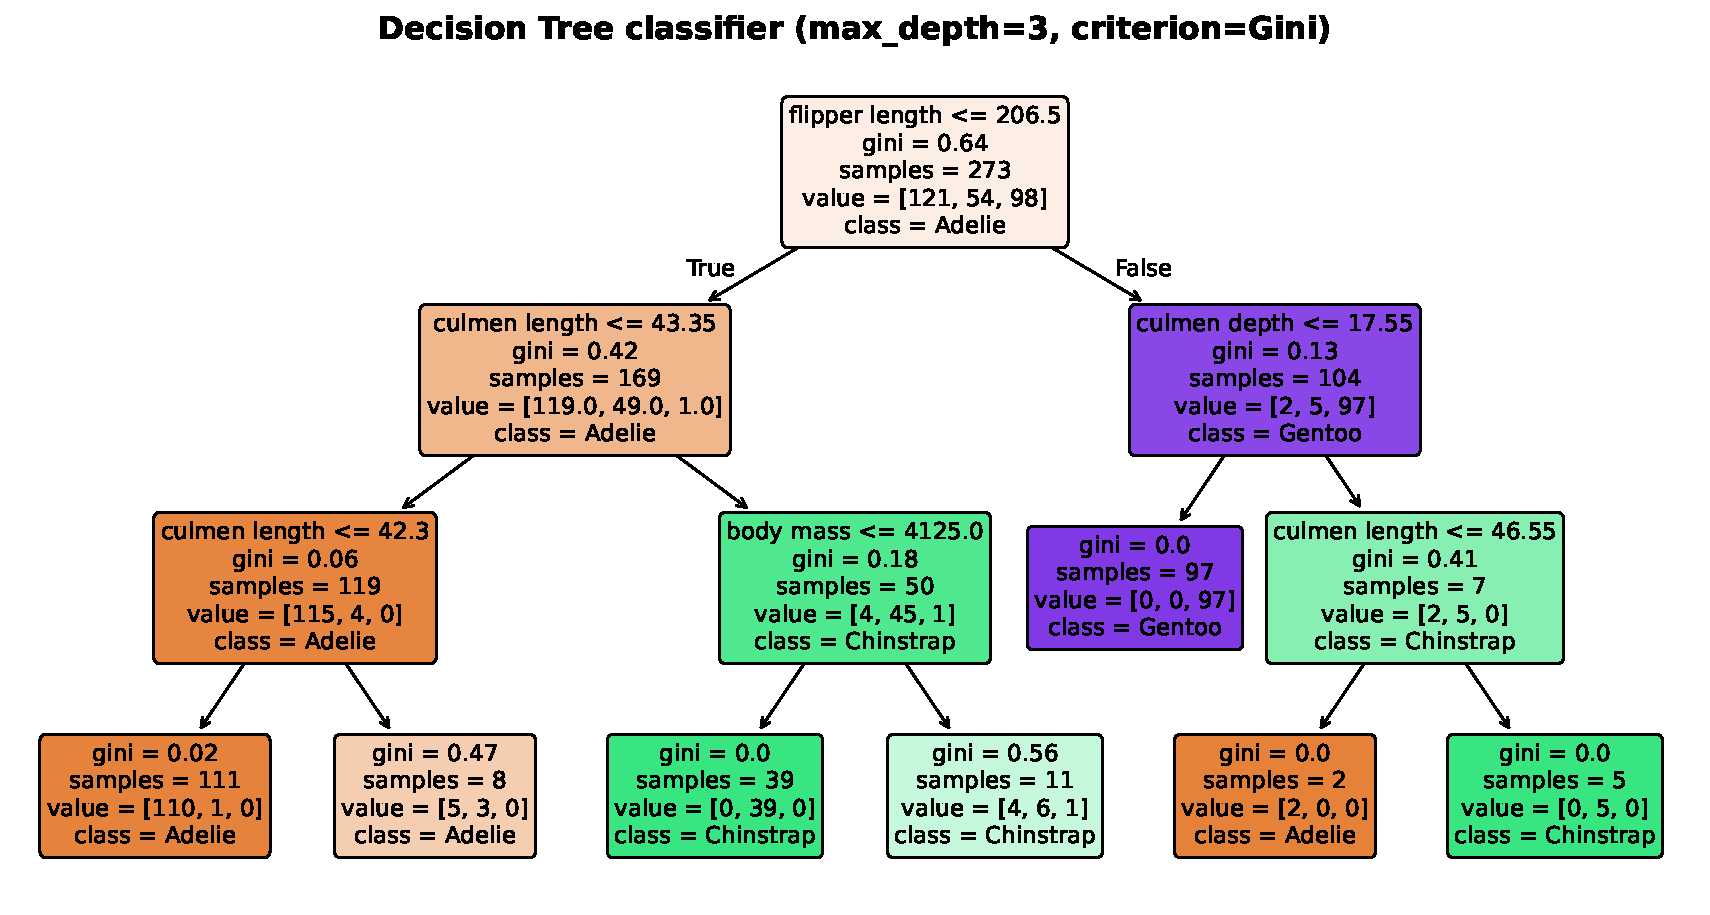
\includegraphics[width=\linewidth]{part4_decision_tree.pdf}
\caption{Decision Tree 主模型。每個節點顯示 split 條件、Gini、samples、各類別筆數與預測 class。}
\end{figure}

這棵樹的實際深度為 3，共有 13 個 nodes 與 7 個 leaves。第一個條件，也就是 root node，使用 \dataterm{flipper\_length\_mm}，threshold 為 206.5 mm：小於等於 206.5 mm 的企鵝走左支，較大的走右支。這個 split 先把多數 Gentoo 和另外兩個物種分開，後面再用 culmen length、culmen depth 與 body mass 繼續細分。

Gini 越低，代表節點裡的 class 越單純。建樹時，模型會尋找能讓子節點加權 Gini 降得最多的候選 split。因此 root 看重的是哪個條件最能分開 training data 中的 species，feature 本身的數值範圍並不會讓它優先被選中。

\section*{3. Manual Prediction Path}
\sectionrule

我從 test set 中挑出 \dataterm{source\_row=3} 的企鵝，手動走一次 prediction path。它的 actual class 是 Adelie，features 如下：

\begin{table}[H]
\centering
\small
\begin{tabular}{lrrrr}
\toprule
 & \textbf{Culmen length} & \textbf{Culmen depth} & \textbf{Flipper length} & \textbf{Body mass} \\
\midrule
Feature value & 39.5 mm & 17.4 mm & 186 mm & 3800 g \\
\bottomrule
\end{tabular}
\end{table}

從 root 開始依序判斷：

\begin{enumerate}[leftmargin=1.8em,itemsep=0.35em]
  \item $\dataterm{flipper\_length\_mm}=186 \leq 206.5$，走左支。
  \item $\dataterm{culmen\_length\_mm}=39.5 \leq 43.35$，再走左支。
  \item $\dataterm{culmen\_length\_mm}=39.5 \leq 42.30$，到達 leaf node 3。
\end{enumerate}

最後到達的 leaf 預測 class 為 Adelie，因此模型的預測和 actual class 相同。從這條 prediction path 也能直接看出，Decision Tree 處理一筆資料時，只需要依序檢查 root 到 leaf 之間的幾個 threshold，整個判斷過程很容易追蹤。

\clearpage
\section*{4. Test-set Performance}
\sectionrule

\begin{figure}[H]
\centering
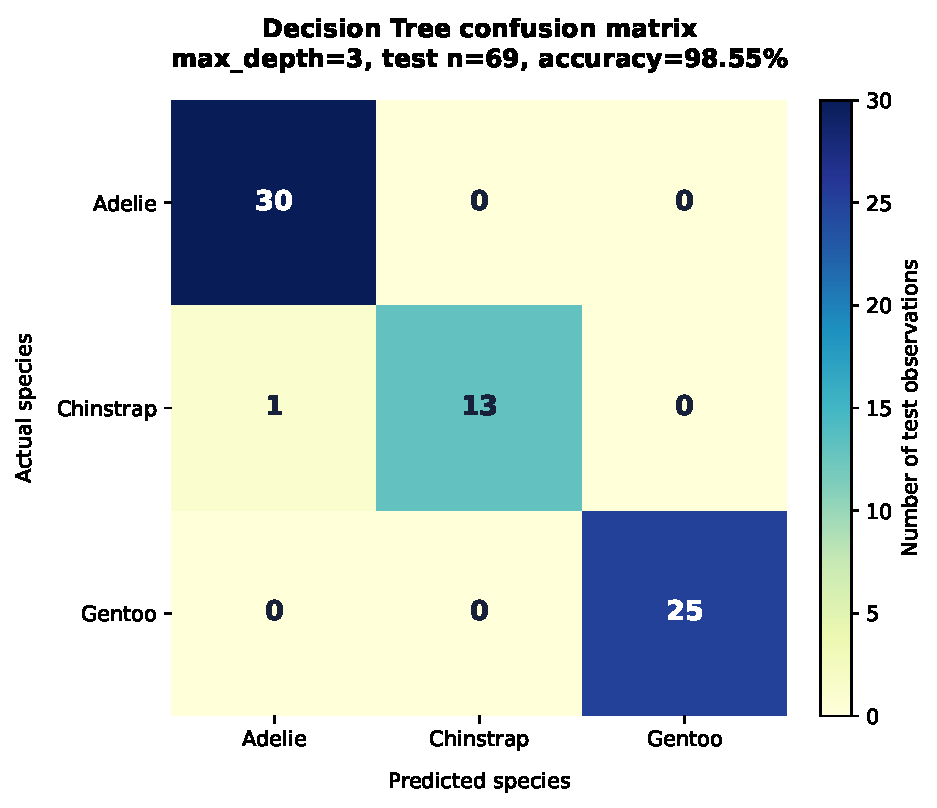
\includegraphics[width=0.69\linewidth]{part4_decision_tree_confusion_matrix.pdf}
\caption{Decision Tree 主模型在固定 test set 的 confusion matrix。列為 actual class，欄為 predicted class。}
\end{figure}

主模型在 69 筆 test data 中判對 68 筆，accuracy 為
\[
\frac{68}{69}=98.55\%,
\qquad
\text{error rate}=1-\frac{68}{69}=\frac{1}{69}=1.45\%.
\]
從 confusion matrix 來看，Adelie 的 30 筆和 Gentoo 的 25 筆全部判對；14 筆 Chinstrap 中則有 13 筆判對，剩下 1 筆被判成 Adelie。唯一的錯誤落在 Adelie 與 Chinstrap 之間，Gentoo 沒有和其他物種混淆。

\section*{5. Small Comparison: Maximum Depth}
\sectionrule

這裡我只調整 maximum depth，其餘資料、criterion 與 random state 都維持不變：

\begin{table}[H]
\centering
\small
\begin{tabularx}{\linewidth}{lrrrrY}
\toprule
\textbf{設定} & \textbf{實際深度} & \textbf{Nodes} & \textbf{Leaves} & \textbf{Accuracy} & \textbf{Test errors} \\
\midrule
$\dataterm{max\_depth}=3$ & 3 & 13 & 7 & 98.55\% & 1 Chinstrap $\rightarrow$ Adelie \\
$\dataterm{max\_depth}=2$ & 2 & 7 & 4 & 98.55\% & 1 Chinstrap $\rightarrow$ Adelie \\
\bottomrule
\end{tabularx}
\end{table}

深度 2 的樹少了 6 個 nodes 與 3 個 leaves，在這組 test set 上卻得到完全相同的 predictions。換句話說，第三層雖然讓 training data 分得更細，對這 69 筆 test data 並沒有帶來實際改善。若只看這次的泛化表現，我會偏向較精簡的深度 2；主模型仍保留作業建議的深度 3，因為它能展示更完整、同時仍然可讀的 tree structure。

\clearpage

\begin{center}
  {\color{accent}\large PART 5}\par
  \vspace{0.25em}
  {\Large\bfseries KNN $\times$ Decision Tree 統整比較}\par
\end{center}

\vspace{1.0em}

\section*{1. How the Two Models Classify}
\sectionrule

KNN 會先用全部四個 features 計算 test object 與 training objects 的距離，再讓最近的 5 個鄰居進行 majority vote。它不會整理出一套明確的全域規則，因此 prediction 很依賴 proximity 如何定義，也會受到各 feature 數值尺度的影響。

Decision Tree 的做法不同。它會在 training data 上逐層選擇一個 attribute 與 threshold，讓切分後的 class 越來越單純。新的 object 從 root 開始，沿著 branches 一路走到 leaf，再由 leaf 給出預測結果。這棵樹的第一個條件是 \dataterm{flipper\_length\_mm}$\leq206.5$；KNN 會同時計算四維距離，tree 每一步則只檢查一個條件。

\section*{2. Proximity and Preprocessing Effects on KNN}
\sectionrule

\begin{table}[H]
\centering
\small
\begin{tabularx}{\linewidth}{L{3.8cm}L{2.6cm}Yrr}
\toprule
\textbf{KNN setting} & \textbf{Scaling} & \textbf{Proximity} & \textbf{Correct} & \textbf{Accuracy} \\
\midrule
Raw Euclidean & 無 & Euclidean & 51 / 69 & 73.91\% \\
Z-score Euclidean & StandardScaler & Euclidean & 69 / 69 & 100.00\% \\
Z-score Manhattan & StandardScaler & Manhattan & 69 / 69 & 100.00\% \\
\bottomrule
\end{tabularx}
\end{table}

Raw Euclidean 直接把四個 feature 的原始數值放進距離計算。由於 body mass 以 g 表示，數值範圍遠大於三個 mm features，很容易主導最後的距離。做完 Z-score 後，每個 feature 都改用各自的標準差衡量，喙部與鰭肢資訊也能更合理地參與鄰居選擇，accuracy 因而從 73.91\% 提高到 100\%。在相同的 Z-score 下，Euclidean 與 Manhattan 對這組 test set 產生完全相同的 predictions。就這次結果而言，scaling 帶來的影響最明顯，$L_1$ 和 $L_2$ 的差別則沒有反映在最終分類上。

\section*{3. How Decision Tree Reacts to the Same Data Scale}
\sectionrule

Decision Tree 使用單一 feature 的排序與 threshold 進行 split，不會把四個 features 的原始數值直接加在一起。正向線性 scaling 會改變 threshold 顯示的數值，但 feature 中各筆觀測的先後次序仍然相同，所以它通常不會像 KNN 一樣，因為單位大小不同就改變分類方式。

結果也呈現出這項差異：同樣使用 raw features，KNN 的 accuracy 是 73.91\%，Decision Tree 則達到 98.55\%。我不會因此認定 tree 在所有資料上都比較好；比較合理的解讀是，這份資料的原始尺度明顯影響 distance-based KNN，而 threshold-based tree 仍能直接利用 flipper length 與 culmen measurements 的切點。對 tree 來說，maximum depth、葉節點最少樣本數和 training data 的變動，才是更直接影響模型結構的因素。

\section*{4. Accuracy and Representative Error Patterns}
\sectionrule

\begin{table}[H]
\centering
\small
\begin{tabularx}{\linewidth}{YrrL{5.7cm}}
\toprule
\textbf{Model} & \textbf{Correct} & \textbf{Accuracy} & \textbf{Errors shown by confusion matrix} \\
\midrule
Raw Euclidean KNN & 51 / 69 & 73.91\% & Chinstrap $\rightarrow$ Adelie 12；Adelie $\rightarrow$ Chinstrap 4；Gentoo $\rightarrow$ Adelie 2 \\
Z-score Euclidean KNN & 69 / 69 & 100.00\% & 無 \\
Decision Tree, depth 3 & 68 / 69 & 98.55\% & Chinstrap $\rightarrow$ Adelie 1 \\
\bottomrule
\end{tabularx}
\end{table}

Z-score KNN 在這組 split 上將 69 筆全部判對，Decision Tree 只多錯 1 筆。不過從模型行為來看，兩者走的是完全不同的路：Tree 用少量且可閱讀的規則完成分類，KNN 則在適當 scaling 後，依靠局部鄰居得到 100\%。Raw KNN 的 confusion matrix 進一步顯示，主要問題是 Adelie 與 Chinstrap 的雙向混淆，而且 Chinstrap 受影響最嚴重；Tree 則把相同類型的錯誤縮小到 1 筆。

\section*{5. Why Accuracy Alone Is Not Enough}
\sectionrule

Accuracy 把所有正確筆數濃縮成一個比例，確實很適合快速比較整體表現，但它不會告訴我錯的是哪個 class，也看不出實際 class 被預測成了什麼。當資料中的類別比例不平均時，少數類別的問題甚至可能被整體 accuracy 蓋過去。Confusion matrix 保留了 actual 與 predicted class 的方向，所以能看出 Raw KNN 的錯誤主要集中在 Chinstrap，也能分清楚 Chinstrap $\rightarrow$ Adelie 與 Adelie $\rightarrow$ Chinstrap 是兩種不同的錯誤。

即使兩個模型的 accuracy 相同，錯誤也可能分布得完全不一樣：一個模型平均錯在各個類別，另一個模型可能幾乎都錯在同一個 class。Part 4 的深度 2 與深度 3 除了 accuracy 相同，confusion matrix 和逐筆 predictions 也完全一致，因此我才會認為它們在這個 test set 上的錯誤型態相同。

\section*{6. Conclusion and Discussion Question}
\sectionrule

做完整份作業後，我覺得 Chapter 2 的 data concepts 和 classification 其實連得很直接。Feature selection 決定模型能看見哪些資訊，data quality 影響輸入是否可靠，train/test split 則讓我能用模型沒參與訓練的資料檢查表現。至於 preprocessing 是否重要，還要看演算法怎麼使用 attributes。KNN 會把 features 組合成距離，所以 scaling 本身就是模型設計的一部分；Decision Tree 依靠單一 attribute 的 threshold 切分，對原始單位較不敏感，但仍然需要控制樹的複雜度。

我最後不會只根據這 69 筆 test data，選出一個「永遠最好」的模型。這次比較真正讓我看到的是，同一份資料交給不同演算法後，KNN 會從「哪些資料彼此接近」出發，Decision Tree 則會尋找「哪些條件最能把類別分開」。把 accuracy、confusion matrix 與模型結構放在一起看，才比較能說清楚結果為什麼會不同。

\textbf{課堂討論問題：}如果未來資料中的 Chinstrap 比例明顯降低，整體 accuracy 可能仍然很高；此時應如何調整評估方式，才能避免忽略少數物種的辨識品質？


\end{document}
